\documentclass[oneside,11pt]{memoir}

\usepackage{microtype}
\usepackage{mathptmx}
\usepackage{graphicx}
\usepackage{amsmath}
\usepackage{bigstrut}
\usepackage{hyperref}
\usepackage{xfrac}
%\usepackage[group-minimum-digits=3,group-separator={,}]{siunitx}
\usepackage{siunitx}

\setverbatimfont{\normalfont\ttfamily\small}

\setsecnumdepth{subsubsection}
\headstyles{bringhurst}
\hypersetup{bookmarksopen,
            bookmarksnumbered,
            colorlinks=true,
            citecolor=red,
            filecolor=red,
            urlcolor=red}

\newsubfloat{figure}
\makepagenote

%-------------------------------------------------------------------------------

\newcommand{\threed}  {3D}
\newcommand{\opengl}  {\textsc{OpenGL}}
\newcommand{\scm}     {\textsc{scm}}
\newcommand{\tiff}    {\textsc{tiff}}
\newcommand{\bigtiff} {Big\textsc{tiff}}
\newcommand{\libtiff} {lib\textsc{tiff}}
\newcommand{\xml}     {\textsc{xml}}
\newcommand{\scmtiff} {\texttt{scmtiff}}
\newcommand{\scmview} {\texttt{scmview}}
\newcommand{\panopath}{\texttt{PANOPATH}}
\newcommand{\rgb}     {\textsc{rgb}}
\newcommand{\mb}    {\,\textsc{mb}}
\newcommand{\vram}    {\textsc{vram}}

\newcommand{\B}{\bigstrut[b]}
\newcommand{\T}{\bigstrut[t]}

\newcommand{\Pos}[1]{\phantom{-}{#1}}
\newcommand{\Neg}[1]{        {-}{#1}}

\newcommand{\inangles}[1]{$\langle$#1$\rangle$}

\newenvironment{optionlist}
  {\setlength{\leftmargini}{1in}\begin{itemize}}{\end{itemize}}

%-------------------------------------------------------------------------------

\begin{document}
\title{Spherical Cube Map TIFF}
\author{Robert Kooima}
\maketitle
\begin{Spacing}{1.1}

% SCMTIFF
%     Many modes

% Example: WAC global ortho blending
% Example: WAC DTM / LOLA merge

% Appendix: Panoview configuration

%------------------------------------------------------------------------------

\chapter{Spherical Cube Map}

\section{Spherical sampling}

The mapping of image data onto the sphere is intuitively similar to a standard \opengl\ cube map. Begin by considering an $n\times n$ raster image applied to the $+Z$ face of a cube. For a spherical cube map, the pixel at row~$r$ and column~$c$ gives a sample at a position $(\alpha, \beta)$ on the sphere, where
\[\alpha=90^{\circ}\,\frac{c + \sfrac{1}{2}}{n} - 45^{\circ}\qquad\beta=90^{\circ}\,\frac{r + \sfrac{1}{2}}{n} - 45^{\circ}.\]
This corresponds to the \threed\ vector
\begin{align*}
x& = \phantom{-}\sin\alpha\, \cos\beta\\
y& =         {-}\cos\alpha\, \sin\beta\\
z& = \phantom{-}\cos\alpha\, \cos\beta.
\end{align*}

This vector has length \(\sqrt{\cos^2\,\alpha + \sin^2\,\alpha\,\cos^2\,\beta}\), but when normalization is required, one will probably prefer the more familiar divisor \(\sqrt{x^2+y^2+z^2}\).

Vectors within the remaining cube faces are simple $90^\circ$ rotations of the definition for $+Z$, trivially implemented in the form of swizzles and negations. For each face, the vector $(x', y', z')$ toward the sample at row and column $(r, c)$ is defined in terms of $(x, y, z)$ as follows.
\begin{center}
\begin{tabular}{rr|r|r|r|r|r}
    &$\Pos{X}$&$\Neg{X}$&$\Pos{Y}$&$\Neg{Y}$&$\Pos{Z}$&$\Neg{Z}$\B\\\hline
$x'=$&$\Pos{z}$&$\Neg{z}$&$\Pos{x}$&$\Pos{x}$&$\Pos{x}$&$\Neg{x}$\T\\
$y'=$&$\Pos{y}$&$\Pos{y}$&$\Pos{z}$&$\Neg{z}$&$\Pos{y}$&$\Pos{y}$\\
$z'=$&$\Neg{x}$&$\Pos{x}$&$\Neg{y}$&$\Pos{y}$&$\Pos{z}$&$\Neg{z}$\\
\end{tabular}
\end{center}

The cube face orientations given by this swizzle table match the definition of a standard \opengl\ linear cube map. It is the non-linear mapping from row and column to 3D vector that puts the ``spherical'' in ``spherical cube map.'' While more expensive to compute, this mapping is more amenable to the delivery of high resolution spherical data sets, as it provides a more uniform tesselation of the sphere, and thus a more consistent density of data at every point on its surface.

As depicted by Figure~\ref{fig:cube}, linear cube map samples stretch in the center of the face and compress toward the edges. While all tessellations of the sphere necessarily demonstrate some degree of similar non-uniformity, the spherical cube map, Figure~\ref{fig:scube}, is visibly closer to the impossible ideal. Specifically, the very smallest samples of a linear cube map, found at the corners, have only $19\%$ of the area of the largest samples at the cube face centers. That is, samples near the center of a cube map face cover more than \emph{five times} the area of samples at the corners. In contrast, the smallest samples of a spherical cube map face, found at the centers of the face edges, have $70\%$ of the area of the largest samples at the face centers.\pagenote{In an unexpected result, as the resolution of an \scm\ page tends toward infinity, the ratio of the solid angle of a center pixel (the largest pixel) to the solid angle of an edge pixel (the smallest pixel) tends toward exactly $\sqrt{2}/2$.} The corner samples of an \scm\ are actually \emph{not} the smallest, with $76\%$ the area of the center samples.

\begin{figure}
  \centering
  \subbottom[Linear cube map]{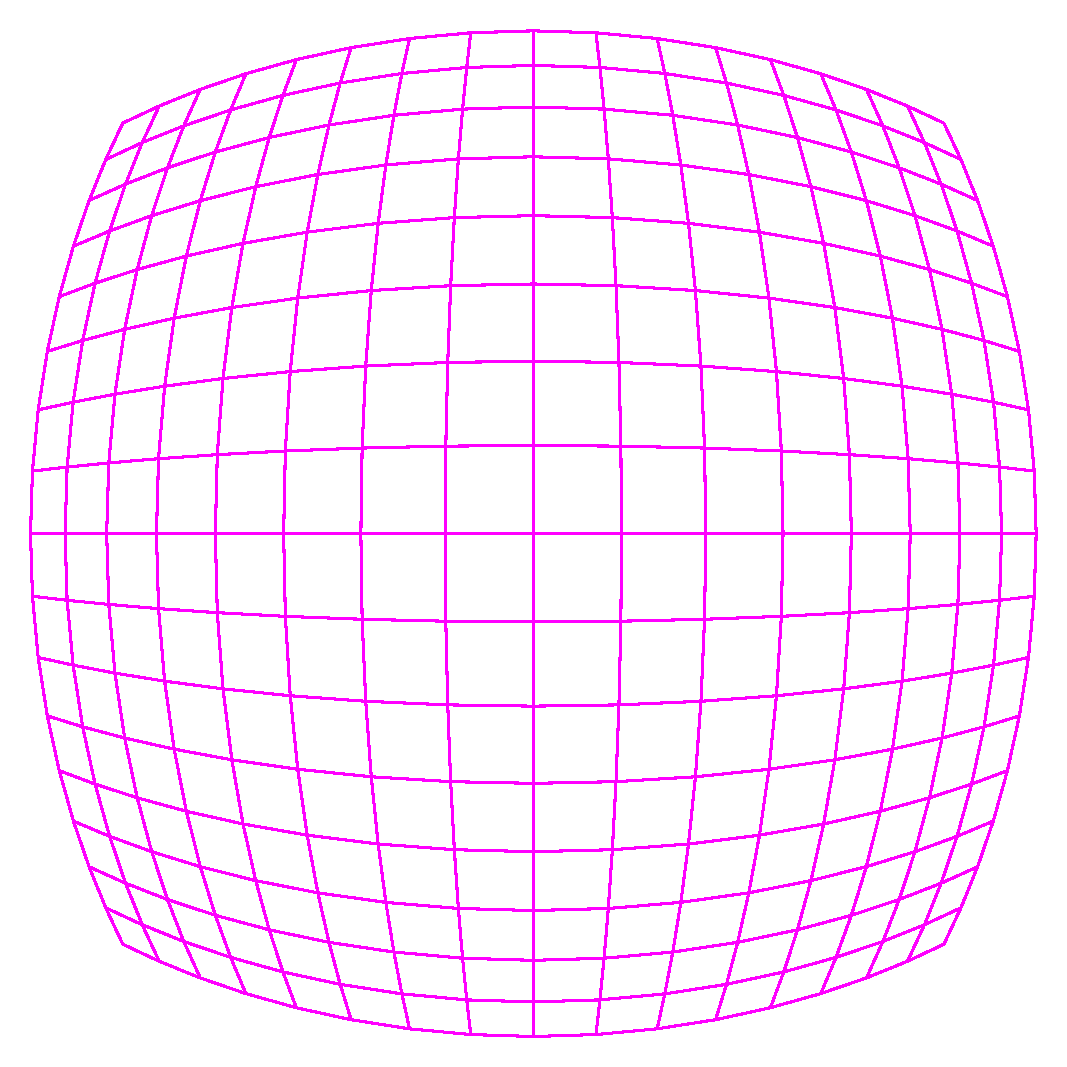
\includegraphics[width=0.3\textwidth]{fig/cube.pdf}\label{fig:cube}}
  \hfil
  \subbottom[Spherical cube map]{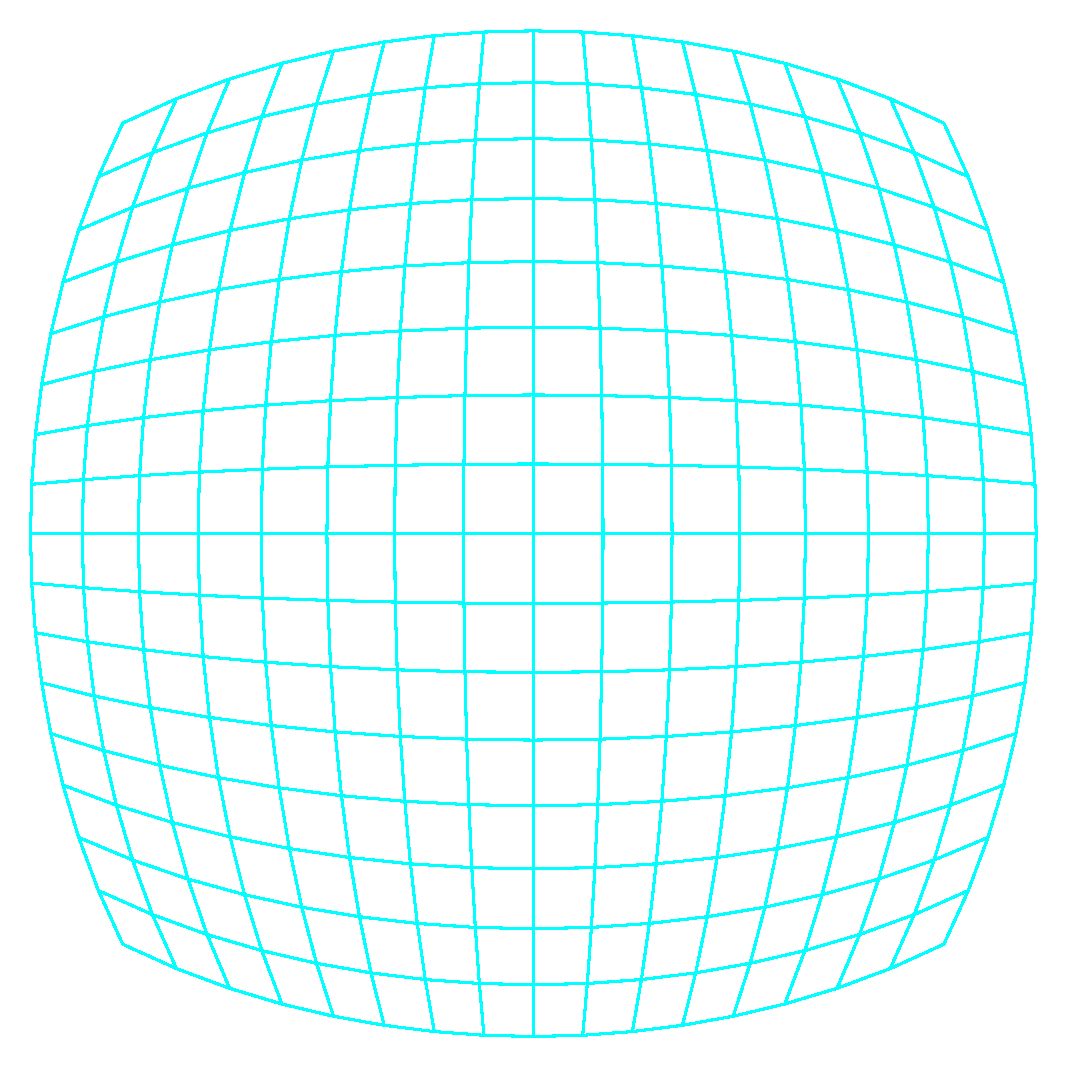
\includegraphics[width=0.3\textwidth]{fig/scube.pdf}\label{fig:scube}}
  \hfil
  \subbottom[Overlaid]{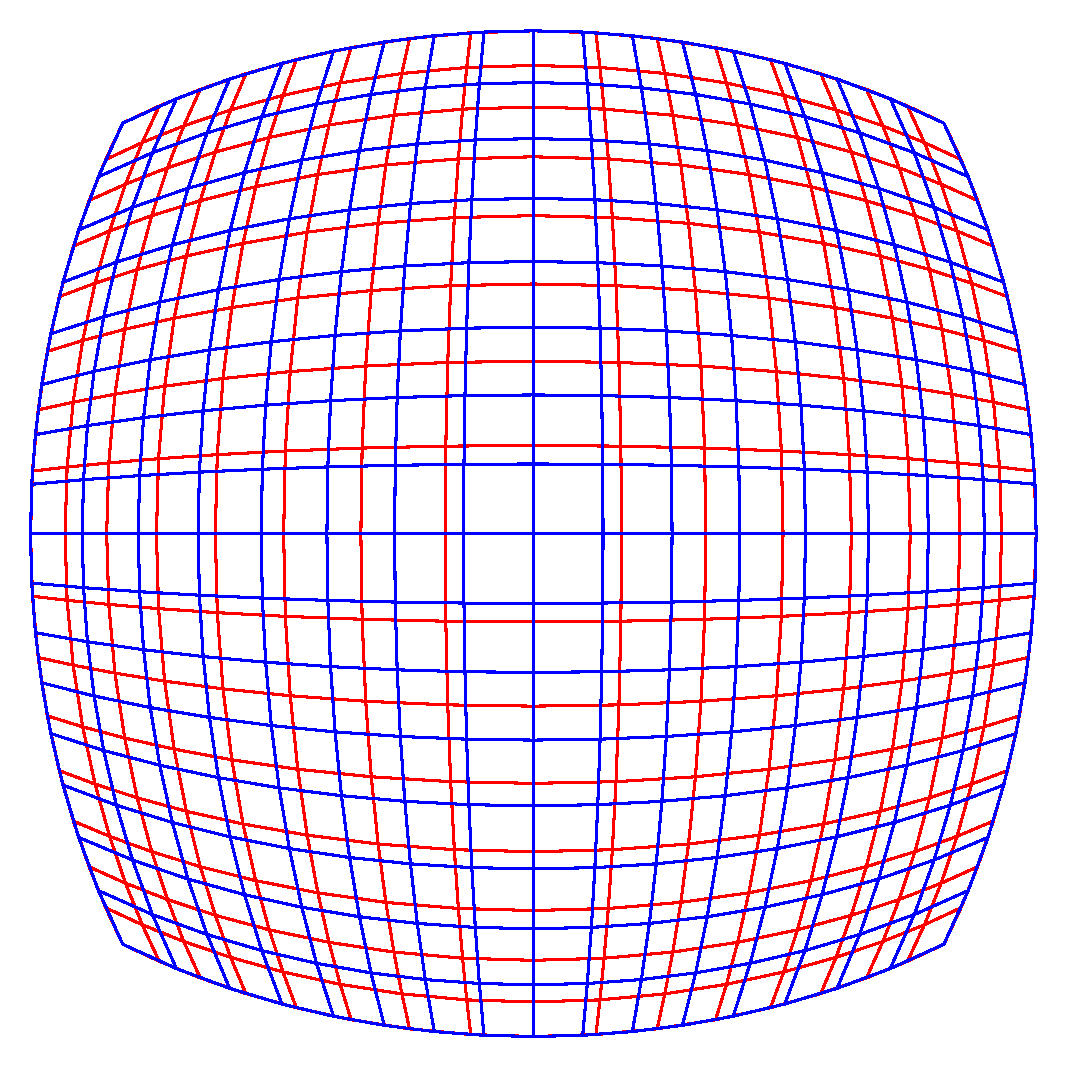
\includegraphics[width=0.3\textwidth]{fig/both.pdf}\label{fig:both}}
  \caption{A comparison of linear and spherical cube map sample uniformity}
  \label{fig:uniformity}
\end{figure}

Similarly, the shortest edge of the linear cube map is only $47\%$ of the length of the longest, while the shortest edge of the spherical cube map is $70\%$ of the length of the longest.\pagenote{Compounding the surprise, the ratio of the length of the shortest edge to the length of the longest edge also tends toward $\sqrt{2}/2$.}  Notably, the vertical and horizontal edges along the center of the \scm\ page all have equal lengths, which means that an \scm\ data set has constant data density along the equator, as well as along the four $90^\circ$ meridians.

\section{Paging}
\label{paging}

While the \scm\ mapping does a good job of uniformly representing data on the surface of the sphere, we're not content to simply map six large images onto the six faces of an inflated cube. Large images are slow to load, and the ultimate objective of the \scm\ data structure is to support real-time viewing with near-instantaneous data access. To render a multi-giga-pixel spherical data set in real-time, an application must calculate frame-by-frame the specific subset of the data visible to the user, as well as the minimum data resolution necessary to fill all pixels of the user's display. Toward that end, the \scm\ represents a large data set in the form of a number of small pages, at a range of resolutions.

The mechanism is akin to a standard \opengl\ mipmap applied to each face of the cube map. Cube faces are recursively subdivided, as shown in Figure~\ref{fig:subdivision}, with each four-sided face cut into four child faces, and the newly-created center vertex placed on the surface of the sphere. Each face of the resulting polyhedron gives one spherically-mapped page of image data. A full \scm\ tree gives \emph{all} levels of detail, up to and including the native resolution of the source data set. The six pages at depth zero (Figure~\ref{fig:cube0}) give low-resolution coverage of the entire sphere. The 24 pages at depth one (Figure~\ref{fig:cube1}) give coverage at twice that density. With each successive increase in depth, the number of pages and the total quantity of image data increases by a factor of four.

\begin{figure}
  \centering
  \subbottom[0]{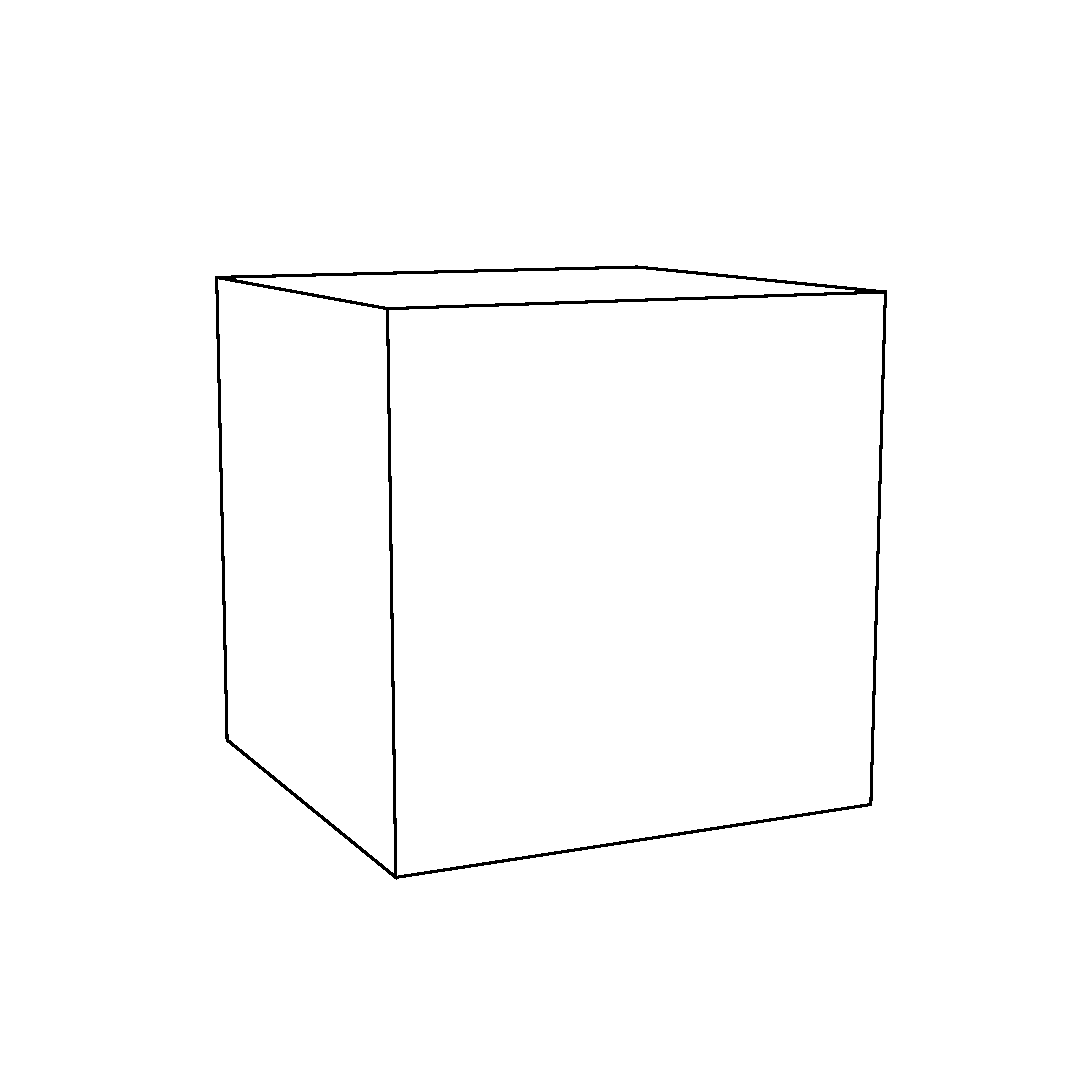
\includegraphics[width=0.18\textwidth]{fig/cube0.pdf}\label{fig:cube0}}
  \subbottom[1]{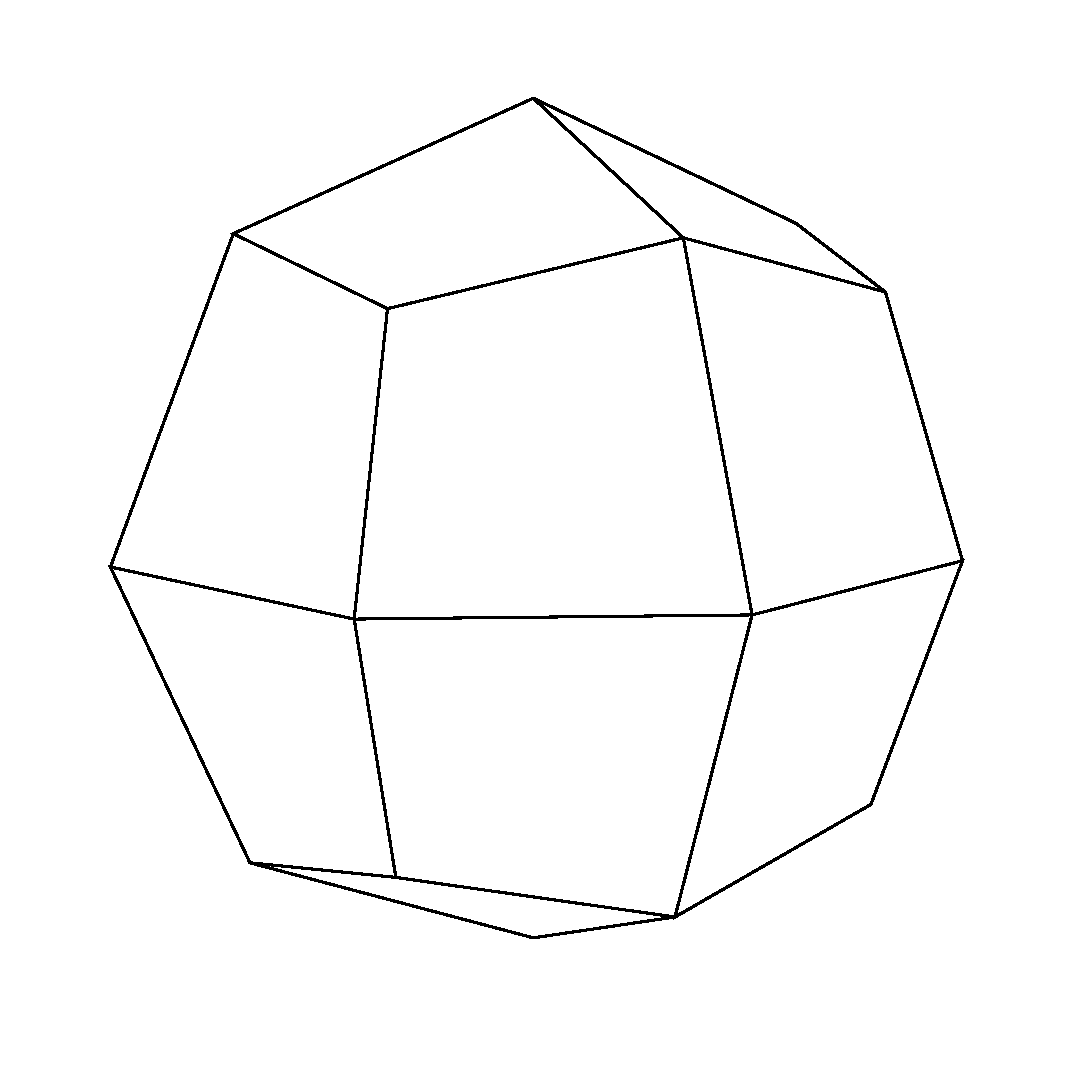
\includegraphics[width=0.18\textwidth]{fig/cube1.pdf}\label{fig:cube1}}
  \subbottom[2]{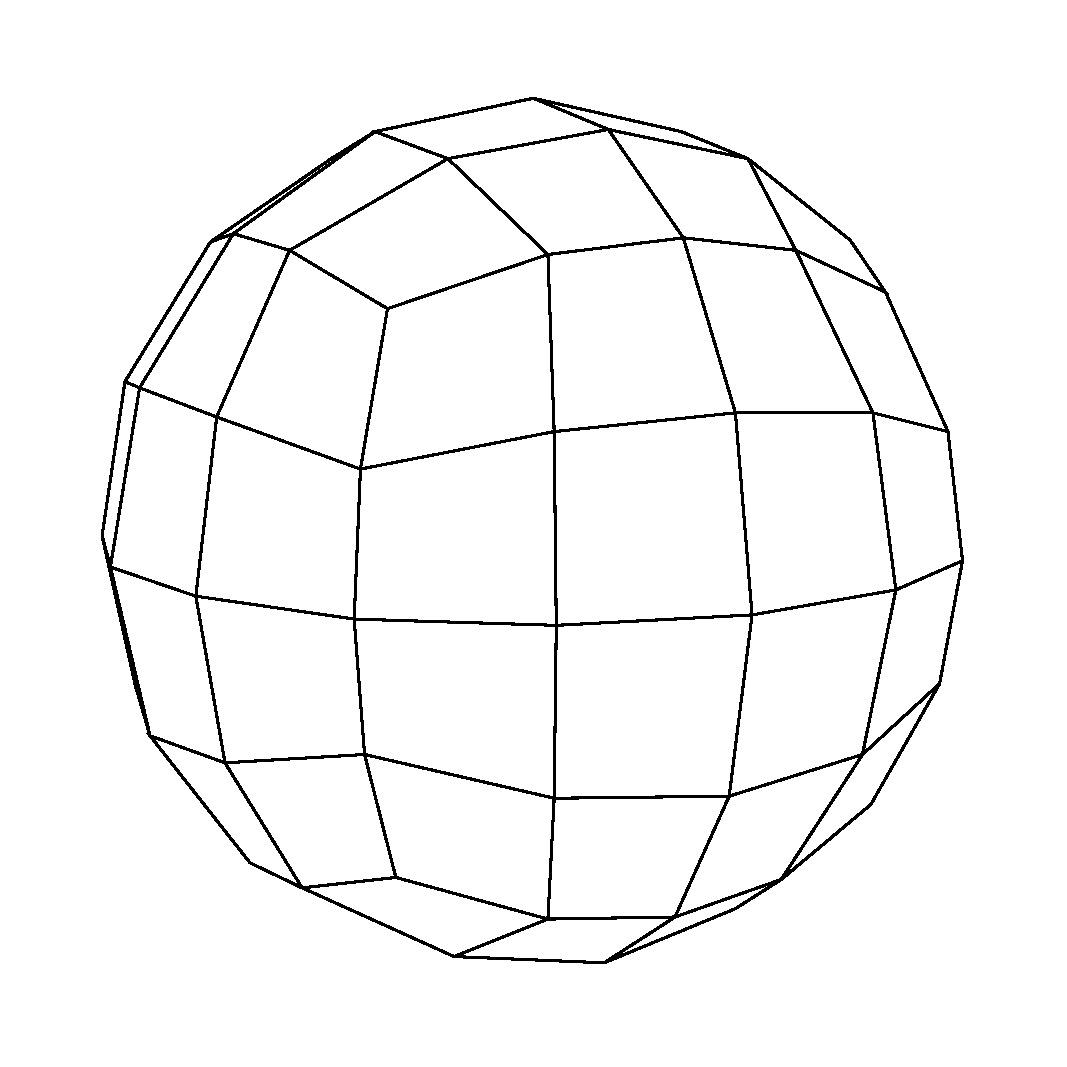
\includegraphics[width=0.18\textwidth]{fig/cube2.pdf}\label{fig:cube2}}
  \subbottom[3]{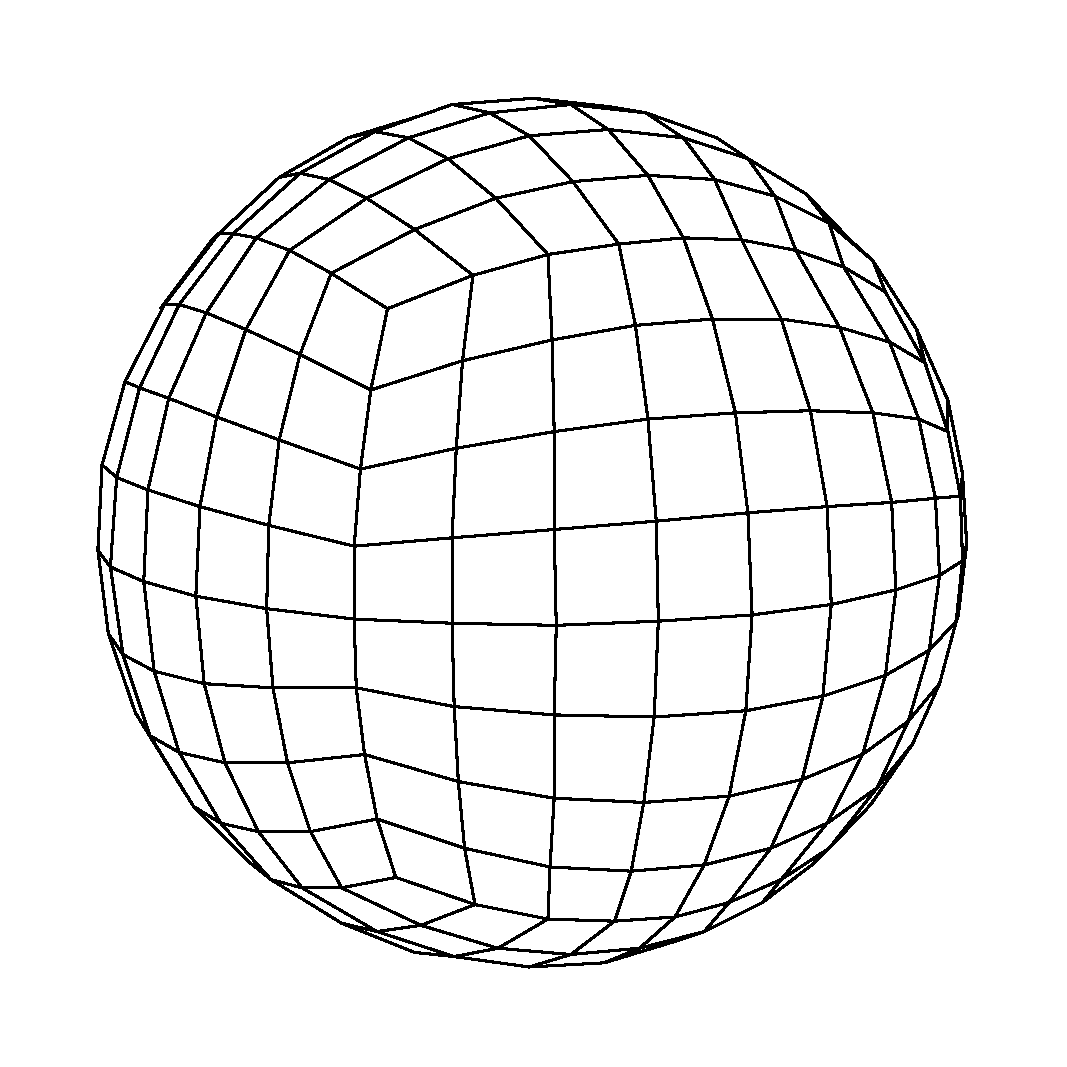
\includegraphics[width=0.18\textwidth]{fig/cube3.pdf}\label{fig:cube3}}
  \subbottom[4]{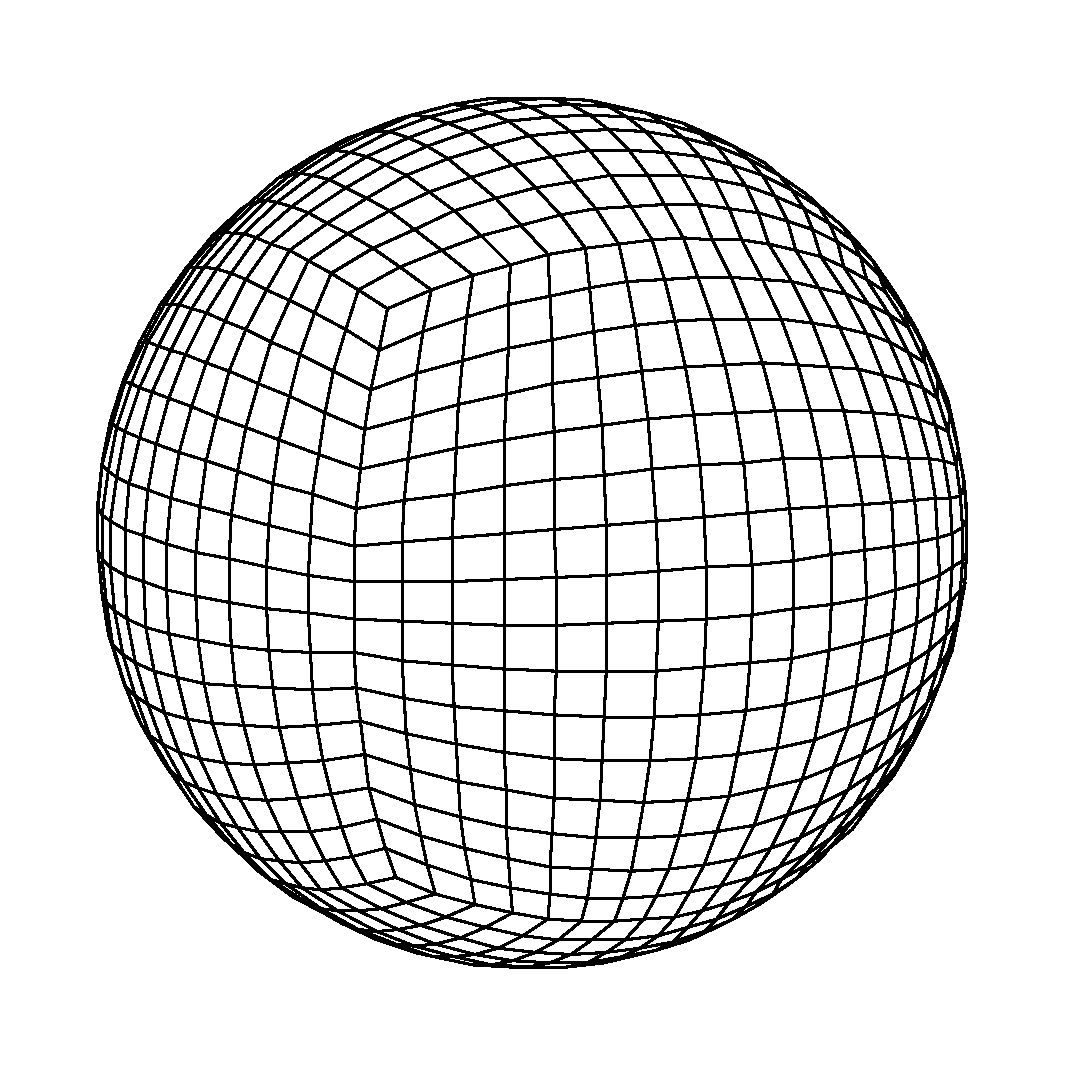
\includegraphics[width=0.18\textwidth]{fig/cube4.pdf}\label{fig:cube4}}
  \hfil
  \caption{Recursive subdivisions of the cube.}
  \label{fig:subdivision}
\end{figure}

Let $d$ be the number of recursive subdivisions applied to the cube. The total number of pages in an \scm\ tree of depth $d$ is
\[m=2^{2\,d+3}-2.\]

Let $n$ be the size in pixels of each page of image data. The effective sphere map resolution of an \scm\ tree with page size $n$ and depth $d$ is
\[w=n\,2^{d+2}\qquad h=n\,2^{d+1}.\]

For reference, Table~\ref{tab:resolution} shows the effective resolutions and page counts of \scm\ trees with depths down to $7$. Page size $n=512$ is often used for power-of-two source images, and $n=720$ works well for geographic and planetary gridded data.

\begin{table}
  \centering
  \label{tab:resolution}
  \begin{tabular}{r|rr|rr|r}
  $d$& $w_{\,512}$& $h_{\,512}$& $w_{\,720}$& $h_{\,720}$& $m$ \B\\\hline
  \num{0}&  \num{2048}&  \num{1024}&  \num{2880}&  \num{1440}&     \num{6} \T\\
  \num{1}&  \num{4096}&  \num{2048}&  \num{5760}&  \num{2880}&    \num{30} \\
  \num{2}&  \num{8192}&  \num{4096}& \num{11520}&  \num{5760}&   \num{126} \\
  \num{3}& \num{16384}&  \num{8192}& \num{23040}& \num{11520}&   \num{510} \\
  \num{4}& \num{32768}& \num{16384}& \num{46080}& \num{23040}&  \num{2046} \\
  \num{5}& \num{65536}& \num{32768}& \num{92160}& \num{46080}&  \num{8190} \\
  \num{6}&\num{131072}& \num{65536}&\num{184320}& \num{92160}& \num{32766} \\
  \num{7}&\num{262144}&\num{262144}&\num{368640}&\num{184320}&\num{131070} \\
  \end{tabular}
  \caption{Effective resolutions and page counts of \scm\ trees with various depths and page sizes.}
\end{table}

Each page is identified by an index between $0$ and $m$ giving the page's position in the breadth-first traversal of the page tree. This index provides a natural ordering for stored pages that maximizes locality of reference and ensures that any prefix of a valid \scm\ is also a valid \scm.

The page index uniquely determines each page's size, position, and orientation on the sphere, and the configuration of the first six root pages determines the layout of the data as a whole. As with all basic definitions shown so far, this root configuration coincides with the definition of a standard \opengl\ cube map. Pages zero through five map onto the faces of a cube as follows.
\[p_0=+X\quad p_1=-X\quad p_2=+Y\quad p_3=-Y\quad p_4=+Z\quad p_5=-Z\]

Much like the classical binary heap data structure, \scm\ tree indices represent positions in a complete tree, and parent-child relationships follow from straightforward integer arithmetic. If page $p_j$ is the parent of page $p_i$ then
\[j=(i-6)/4.\]

If page $p_i$ is the $k$th child of page $p_j$ then
\[i=6+4\,j+k\]

The child order $k$ of page $p_i$ is
\[k=(i-6)-4\,((i-6)/4).\]

The \scm\ tree level $l$ at which page $p_i$ appears is
\[l=\frac{\lfloor\log_2\,(i+2)\rfloor - 1}{2}\]

When processing and rendering \scm\ data, it is often necessary for applications to determine the indices of spatially adjacent pages. This relationship does not emerge readily, and is somewhat more challenging to compute. An implementation, provided in the source, has complexity linear in the distance to the adjacent pages' first common ancestor.

%------------------------------------------------------------------------------

\chapter{\scm\ Pre-processing}

\section{SCMTIFF Usage}

Spherical data sets in a variety of image formats are converted to \scm\ \tiff\ files by the \scmtiff\ utility. Given the variety of source data preparations, this conversion involves multiple steps, and is often directed by a script or build system. \scmtiff\ is a multi-tool that implements all of the different processes needed when traversing the path from raw data to usable \scm. It takes three global options followed by a list of per-process options and a list of input files.

\bigskip\noindent\scmtiff\ \texttt{-p} \inangles{\textit{process}} [\texttt{-o} \inangles{\textit{output}}] [\textit{options}] \inangles{\textit{input}} [\ldots]

\begin{optionlist}
\item[\texttt{-p} \inangles{\textit{process}}] Selects the \scm\ process. Alternatives include \texttt{convert}, \texttt{combine}, \texttt{mipmap}, \texttt{border}, \texttt{catalog}, and \texttt{normal}. Each of these processes is described here, and examples of complete conversions are given below.

\item[\texttt{-o} \inangles{\textit{output}}] Gives the name of the output file. If left unspecified, the default is \texttt{out.tif}, unless otherwise noted.

\item[\texttt{-T}] Requests that process timing be collected and printed to the terminal upon completion.
\end{optionlist}

An \scm\ \tiff\ file produced by the \scmtiff\ tool is a standard \bigtiff\ image, suitable for processing using any \bigtiff-compatible tool. Notably, this includes \libtiff\ version 4 or later, and its related utilities.\pagenote{It should be noted that a number of the \scm\ \tiff\ fields reference embedded data by offset. Whenever possible, this data is embedded exactly once, despite being referred-to by fields in all directories. Applications that copy \tiff\ data should be careful not to replicate this data, as one such field, the page catalog \texttt{0xFFB1}, can be several megabytes in size. Indeed, directory extractions and other heavy modifications to a \tiff\ file structure will invalidate the page catalog anyway.}

\subsection{Convert}

\noindent\scmtiff\ \texttt{-p convert} [\texttt{-o} \inangles{\textit{output}}] [\textit{options}] \inangles{\textit{input}} [\ldots]

\bigskip The \texttt{convert} process is the first and most basic, taking source data input and producing \scm\ \tiff\ output. Source data with a full-sphere equirectangular projection may be provided in \textsc{jpeg}, \textsc{png}, or \textsc{tiff} format, with up to four channels. Data with more complex projection may be provided in \textsc{pds} format, as attached-label \textsc{img} files or detached-label \textsc{lbl}~/~\textsc{img} pairs. Channels may have 8 or 16-bit signed or unsigned integer samples, or 32-bit floating point samples.

If the output file name is not specified using the \texttt{-o} option to \scmtiff, the default name is generated by replacing the file extension of the input file name with \texttt{.tif}. This is important when multiple input files are given on a single command line.\pagenote{Yes, this process is dumb enough to overwrite a source data file that already has the \texttt{.tif} extension.}

\texttt{convert} has the most options of any process, as the parameters specified at the first step are carried through into the final data product.

\begin{optionlist}
\item[\texttt{-n} \inangles{$n$}] Gives a value for $n$, the \scm\ page size. Default is $512$.

\item[\texttt{-d} \inangles{$d$}] Gives a value for $d$, the \scm\ tree depth. Default is $0$. See Section~\ref{paging} for definitions and examples of how the selection of $n$ and $d$ affect image resolution and file size.

\item[\texttt{-b} \inangles{$b$}] Overrides the number of bits per channel. By default, \scmtiff\ uses the bit depth specified by the input image file. If a change in bit depth is desired, this value $b$ is used instead. Values of $8$ and $16$ select integer samples and $32$ selects floating point samples.

\item[\texttt{-g} \inangles{$g$}] Overrides the signedness of integer data. By default, \scmtiff\ uses the type specified by the input file, but if a change is desired, $0$ specifies unsigned and $1$ signed. This option has no effect if floating point samples are selected.

\item[\texttt{-t} \inangles{\textit{file}}] Specifies a text file containing an image description. The contents of this file are read and embedded in the generated \tiff\ file. Subsequent \scmtiff\ processes do retain this text and do not take a separate description option. Thus, any description of the final data product should be fully specified in the initial \texttt{convert} process.

\item[\texttt{-N} \inangles{$n_0$}\texttt{,}\inangles{$n_1$}] Specifies a normalization range. Unsigned integer samples have a natural normalized range of $(0, 1)$, signed integer samples have the normalized range of $(-1,1)$, and floating point samples have the full range of a 32-bit float. This option remaps each sample onto the range $(n_0,n_1)$. The choice of normalization depends largely on the character of the input and the type of the output. The default normalization retains the natural range of the data.

\item[\texttt{-L} \inangles{$\lambda_c$}\texttt{,}\inangles{$\lambda_0$}\texttt{,}\inangles{$\lambda_1$}] Specifies a longitudinal mask. This causes data to appear over a given range of longitudes, fading out at the edges, thus allowing the blended combination of separate source data files. This option chooses a range of degrees centered at $\lambda_c$, extending to $\lambda_c\pm\lambda_1$, and fading with cubic drop-off to $\lambda_c\pm\lambda_0$.

\item[\texttt{-P} \inangles{$\phi_c$}\texttt{,}\inangles{$\phi_0$}\texttt{,}\inangles{$\phi_1$}] Specifies a latitudinal mask. This option chooses a range of degrees centered at $\phi_c$, extending to $\phi_c\pm\phi_1$, and fading with cubic drop-off to $\phi_c\pm\phi_0$. Longitudinal and latitudinal masks may be applied simultaneously.
\end{optionlist}

\subsection{Combine}

\noindent\scmtiff\ \texttt{-p combine} [\texttt{-o} \inangles{\textit{output}}] [\textit{options}] \inangles{\textit{input}} [\ldots]

\bigskip The \texttt{combine} process is the second step in cases where a data set is provided in a form spread across multiple data file. It merges multiple converted \scm\ \tiff\ input files into a single \scm\ \tiff\ output file. It takes just one optional argument.

\begin{optionlist}
\item[\texttt{-m} \inangles{\textit{mode}}] Specifies the operator mode used to combine samples. The \texttt{max} mode selects the largest sample from each of the named files. The \texttt{sum} mode is the default and sums all named files. The \texttt{max} mode is often used when merging data sets of differing projection, while the \texttt{sum} mode is used when combining data sets that have had a longitudinal or latitudinal mask applied in the \texttt{convert} process.
\end{optionlist}

\subsection{Mipmap}

\noindent\scmtiff\ \texttt{-p mipmap} \inangles{\textit{input}}

\bigskip The \texttt{mipmap} process generates the intermediate nodes of an \scm\ tree. In general, the \texttt{convert} process generates tree leaves, the \texttt{combine} process merges trees, and the \texttt{mapmap} process subsamples the result, enabling real-time display of the data at arbitrary resolution. It is important to \texttt{combine} before \texttt{mipmap}ping, as boundary artifacts may remain apparent in the intermediate pages of combined mipmaps.

The \texttt{mipmap} process takes no parameters. In the interest of efficiency, mipmapping occurs \textit{in place}. The output file name option is ignored and subsampled pages are appended to the existing file. The \texttt{mipmap} process generates as many subsampled levels as possible, and in the common case, an input with depth $d$ will have $d-1$ levels appended to it.

\subsection{Border}

\noindent\scmtiff\ \texttt{-p border} [\texttt{-o} \inangles{\textit{output}}] \inangles{\textit{input}}

\bigskip In truth, an \scm\ with page size $n$ is stored in a \tiff\ file with image width and height $n+2$. The \texttt{border} process fills these extra pixels in the outermost rows and columns of each page with pixels from the adjacent rows or columns of the four neighboring pages. This provides each page with the context needed by the graphics hardware to perform linear magnification filtering across page boundaries, effectively allowing many small images to appear as a single very large image.\pagenote{The replicated borders provide only a single pixel of context. This enables linear magnification filtering, but does \emph{not} enable anisotropic filtering.} If this step is not performed, artifacts will appear in the output. In practice, the \texttt{border} process is expensive, as it must decompress and recompress every page of the \scm.

\subsection{Catalog}

\noindent\scmtiff\ \texttt{-p catalog} \inangles{\textit{input}}

\bigskip The \texttt{catalog} process generates a sorted array of index-offset pairs that allow an \scm\ rendering application to immediately determine exactly where each page appears in the \scm\ \tiff\ file. Such applications are usually aware of how points on the sphere map onto indices, and thus the page catalog generated by the \texttt{catalog} process allows applications to straightforwardly locate the unique \scm\ \tiff\ data that maps onto any point on the sphere at any resolution. In the absence of this catalog, an \scm\ application must scan the file for indices, noting offsets as it goes. This heavily I/O-bound process often incurs significant delays and impedes real-time, interactive display.

Like mipmapping, the \texttt{catalog} process takes no parameters and occurs \emph{in place}. The output file name option is ignored and the catalog data is appended to the input file.

\subsection{Normal}

\noindent\scmtiff\ \texttt{-p normal} [\texttt{-o} \inangles{\textit{output}}] [\textit{options}] \inangles{\textit{input}}

\bigskip The \texttt{normal} process computes a normal map for a given height map. The input may have any number of channels and any format, but only the first channel is used, and the normalization of that channel is modified by the range of radii specified by the command line option. The output will always have 3 channels of 8-bit unsigned samples, scaled and biased to $(0,1)$ as is standard practice in normal mapping, though the normals are given in \emph{object} space rather than \emph{tangent} space.

Regardless of whether the input height map was bordered or cataloged, the output normal map will be neither bordered nor cataloged. In contrast, a mipmapped input height map \emph{will} produce a mipmapped normal map output, and indeed one should \emph{always} normalize mipmaps instead of mipmapping normals, as a mipmapped normal is not guaranteed to have unit length.

\begin{optionlist}
\item[\texttt{-R} \inangles{$r_0$}\texttt{,}\inangles{$r_1$}] Specifies the true range of radii represented by the normalized height map input. This allows the true magnitude of the \emph{change} in height to be computed, which gives slope, which gives the normal vector.
\end{optionlist}

\section{SCMVIEW Usage}

The secondary utility \scmview\ enables inspection and side-by-side comparison of \scm\ \tiff\ output.

\section{SCMTIFF Examples}

The most straightforward SCM TIFF process uses a simple image file giving an equirectangular spherical projection, such as that shown in Figure~\ref{fig:bluebonnet}. This image is $32768\times 16384$ with 3 channels of 8-bit unsigned samples. Its name reflects that it was captured at the Bluebonnet Swamp Nature Center, it was the first of several captures, and it gives the left channel of a stereoscopic pair.

\begin{figure}
  \centering
  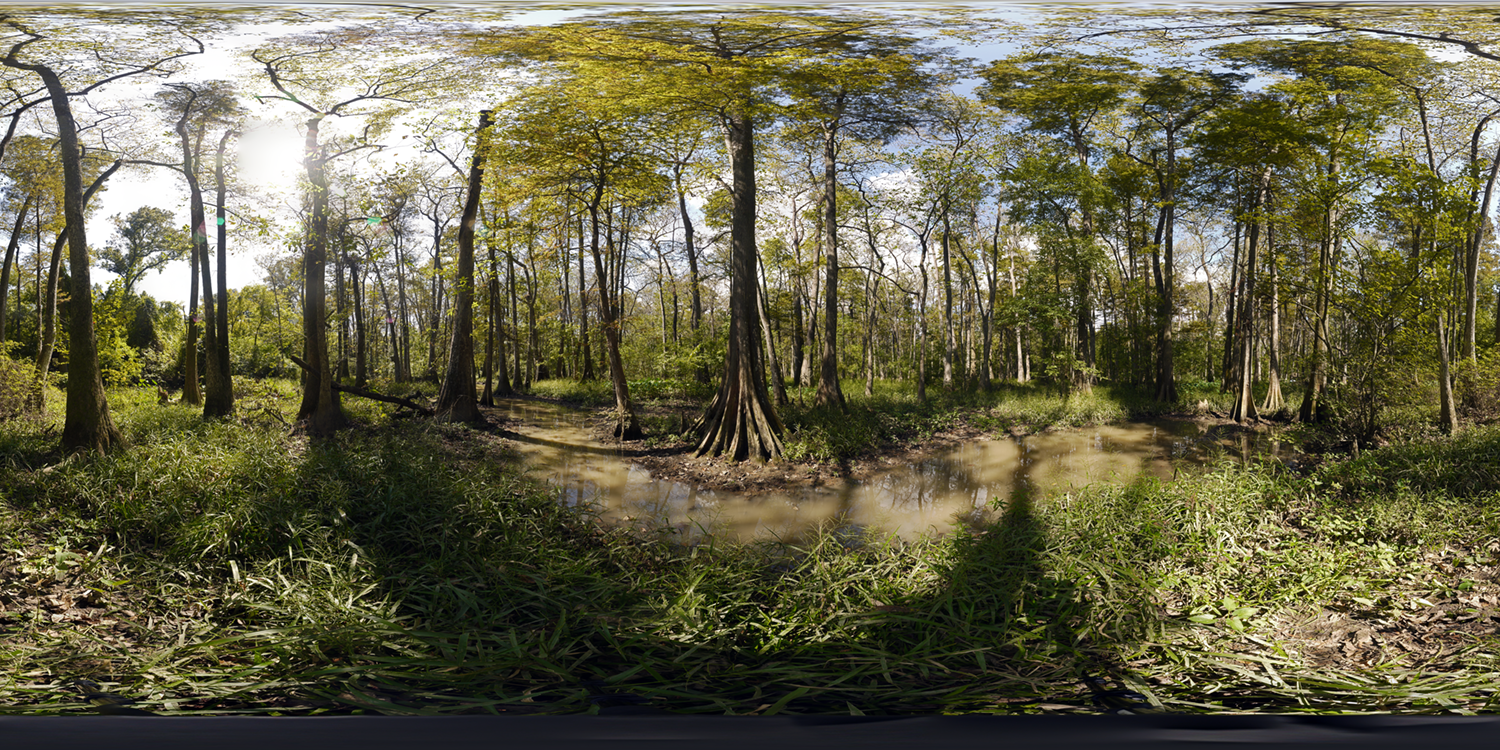
\includegraphics[width=\textwidth]{fig/bluebonnet.png}
  \caption{\texttt{Bluebonnet-0-L.tif}, an equirectangular full-sphere panorama}
  \label{fig:bluebonnet}
\end{figure}

A brief description is added to an ASCII text file named \texttt{desc.txt}.

\begin{verbatim}
Bluebonnet Swamp Nature Center - 9 October 2011
Copyright (c) 2011 Robert Kooima
\end{verbatim}

Table~\ref{tab:resolution} indicates that an image with this resolution is well-represented by an \scm\ with page size $n=512$ and depth $d=4$. When finished, this \scm\ will have $2046$ pages. The first step is to run the \texttt{convert} process to generate the leaves of this tree. The output file name is chosen to reflect the parameters of the \scm\ as well as the state of its processing. This convention is optional.

\begin{verbatim}
scmtiff -T -p convert -n 512 -d 4 -t desc.txt
        -o Bluebonnet-0-L-512-4-M.tif Bluebonnet-0-L.tif
\end{verbatim}

If the output is examined using \scmview, pages $510$ through $2045$ will be present with a resolution of $514\times 514$. Image detail will closely reflect that of the input. There will be mild projection distortion apparent is some pages, though the degree of distortion will be far less than that at the top and bottom of the equirectangular input. All pages will have a ring of black pixels around the outside.

The second stop is to run the \texttt{mipmap} process on this output to generate the intermediate, subsampled pages.

\begin{verbatim}
scmtiff -T -p mipmap Bluebonnet-0-L-512-4-M.tif
\end{verbatim}

Examination with \scmview\ will show that pages $0$ through $2045$ are now all present. Pages $0$ through $5$ will show wide views in each of the cardinal directions, and pages $2$ and $3$ will show nicely recovered polar views with all of the projection distortion in the input rectified.

Third, the border pixels must be filled with adjacent page information. This process alters the compressed size of each page, and cannot be performed in-place. Thus, an output file name is required and a new \scm\ \tiff\ file is generated.

\begin{verbatim}
scmtiff -T -p border
        -o Bluebonnet-0-L-512-4.tif Bluebonnet-0-L-512-4-M.tif
\end{verbatim}

The output is a complete \scm\ tree. Figure~\ref{fig:sixfaces} shows the first six pages generate from Figure~\ref{fig:bluebonnet}.

\begin{figure}
  \centering
  \subbottom[0]{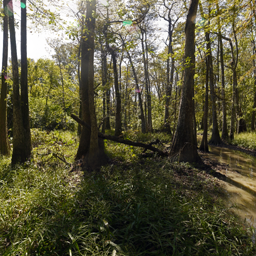
\includegraphics[width=0.15\textwidth]{fig/bluebonnet0.png}}
  \subbottom[1]{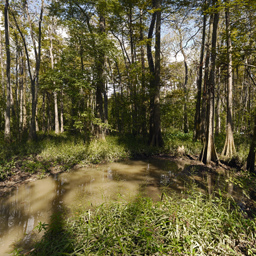
\includegraphics[width=0.15\textwidth]{fig/bluebonnet1.png}}
  \subbottom[2]{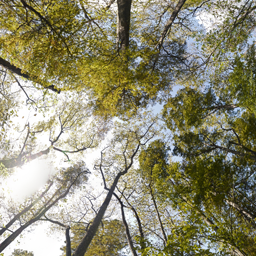
\includegraphics[width=0.15\textwidth]{fig/bluebonnet2.png}}
  \subbottom[3]{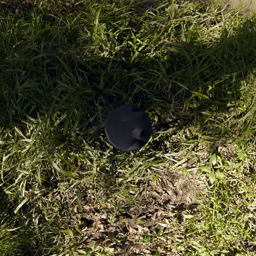
\includegraphics[width=0.15\textwidth]{fig/bluebonnet3.png}}
  \subbottom[4]{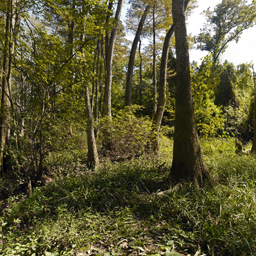
\includegraphics[width=0.15\textwidth]{fig/bluebonnet4.png}}
  \subbottom[5]{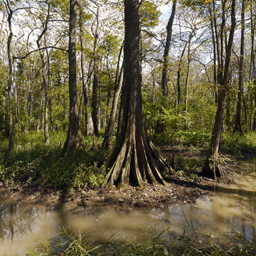
\includegraphics[width=0.15\textwidth]{fig/bluebonnet5.png}}
  \caption{The six root pages of the Bluebonnet \scm.}
  \label{fig:sixfaces}
\end{figure}


%------------------------------------------------------------------------------

\chapter{\scm\ Interactive Display}

\section{Render Library}

The out-of-core panorama renderer is implemented as a small C++ library that may be embedded within any \opengl\ host application. This library has just one system-level configuration parameter:

\panopath\ is a shell environment variable akin to the bash executable path. It lists directories where spherical cube map \tiff\ files may be found. If the application requests that the renderer load a file, but the renderer cannot find that file, then it will search this list of directories. Set this variable in the shell resource file, as need be, separated by colons. For example,

\begin{verbatim}
export PANOPATH=/share/pan:$HOME/data/pan:.
\end{verbatim}

For cluster-driven display systems, try to replicate all panorama image files to local directories on all rendering nodes. This will perform better than data files stored on network shares.

\section{Panorama Definition File}

An example panorama viewer, panoview, is implemented using the Thumb framework. While the previous sections on panorama handling apply to any embedding of the panorama renderer, the following sections describe the configuration and usage specifically of panoview.

For correct display, panoview must understand the parameters of each panoramic image. The panorama definition is an \xml\ file that provides this information.

Like any data file, Thumb must be able to find these panorama definitions. They are appear in the Thumb data hierarchy like any other configuration file. This means they may be placed in a data directory rooted at the current directory, or in the ~/.thumb hierarchy, or in a data hierarchy given by the \texttt{THUMB\_RO\_DATA} environment variable. Panorama definition files need not be stored along side the \tiff\ files that the reference. It is the \panopath\ environment variable that defines the location of these.

\subsection{Basic Stereo Panorama}

Here is an example of a basic stereo panorama definition, named Blue-Mounds-8.xml.

\begin{verbatim}
<?xml version="1.0"?>
  <panorama channels="2" depth="4" size="512"
      mesh="16" height="0" radius="6"
      vert="glsl/sph-zoomer.vert"
      frag="glsl/sph-render.frag">
  <image channel="0" file="Blue-Mounds-8-L-512-4.tif" />
  <image channel="1" file="Blue-Mounds-8-R-512-4.tif" />
  </panorama>
\end{verbatim}

The file begins with an \xml\ header and contains a single root panorama element with several attributes and one image sub-element for each panorama image.

The channels attribute gives the number view positions. This adapts a panorama definition to a specific display configuration. A desktop display will have one channel, a CAVE will have two, and a multi-view lenticular may have many more.

The size and depth attributes give the size of each page in the panorama image files and the depth of their page hierarchies. Note that the values coincide with the image parameters given by the file names. Other values are allowed, and may enable quality-speed tradeoffs.

The mesh attribute determines the tesselation of the geometry mesh used to render each page of data. The example value, 16, indicates that each page of the sphere will be rendered using a $16\times 16$ grid of polygons. There is little reason to change this.

The radius attribute determines the radius of the spherical proxy geometry used to render the panorama. The height attribute determines the placement of the proxy geometry in the scene, and should match the height of the camera at the time the panorama was captured. These values are given in meters, and are mostly significant in VR display environments. The default radius is 6 meters, and the default height is 0 meters.

The vert and frag attributes give the vertex and fragment programs to be used by the renderer, named relative to the root of the Thumb data hierarchy. These will remain the same for most panorama definitions.The zoomer; vertex program must be specified for zoomable panoramas. The render fragment program is used for static panoramas such as this one.

\subsection{Multi-image Panorama}

The following example, Taliesin-Path, is more complex. It defines several images for each channel. This will behave as a circular list of images, and the renderer will interpolate between them in order, following an internal “playback head.”

\begin{verbatim}
<?xml version="1.0"?>
  <panorama channels="2" depth="3" size="512"
      vert="glsl/sph-zoomer.vert"
      frag="glsl/sph-blend.frag">
  <image channel="0" file="Taliesin-Path-A-L-512-3.tif" />
  <image channel="1" file="Taliesin-Path-A-R-512-3.tif" />
  <image channel="0" file="Taliesin-Path-B-L-512-3.tif" />
  <image channel="1" file="Taliesin-Path-B-R-512-3.tif" />
  <image channel="0" file="Taliesin-Path-C-L-512-3.tif" />
  <image channel="1" file="Taliesin-Path-C-R-512-3.tif" />
  <image channel="0" file="Taliesin-Path-D-L-512-3.tif" />
  <image channel="1" file="Taliesin-Path-D-R-512-3.tif" />
  <image channel="0" file="Taliesin-Path-E-L-512-3.tif" />
  <image channel="1" file="Taliesin-Path-E-R-512-3.tif" />
  <image channel="0" file="Taliesin-Path-F-L-512-3.tif" />
  <image channel="1" file="Taliesin-Path-F-R-512-3.tif" />
  <image channel="0" file="Taliesin-Path-G-L-512-3.tif" />
  <image channel="1" file="Taliesin-Path-G-R-512-3.tif" />
  <image channel="0" file="Taliesin-Path-H-L-512-3.tif" />
  <image channel="1" file="Taliesin-Path-H-R-512-3.tif" />
  </panorama>
\end{verbatim}

Note that the frag attribute of the panorama element specifies the blend fragment program. This program performs the interpolation. Non-interpolating panoramas should use the \texttt{sph-render.vert} program, as \texttt{sph-blend.vert} doubles the texture access load of the renderer.

\section{Panoview Usage}

Panoview is configured and run like any other Thumb application. The following keyboard commands are defined.

\begin{itemize}
\item[F1] Toggle the panoview file selection dialog. This dialog allows the user to navigate the Thumb data hierarchy and select a panorama definition for viewing.

\item[F2] Toggle the cache visualization overlay. This allows the set of all resident pages to be viewed in thumbnail.

\item[F3] Toggle the page coloration debug view. This feature recolors each incoming page to indicate its depth in the page tree.

\item[F4] Toggle automatic zoom centering. This option controls whether the center of the zoom is static or dynamic.
\end{itemize}

In addition, there is one option in the Thumb configuration file conf.xml that impacts the behavior and performance of the panorama renderer.

% Probably want to rename everything from "sph" to "scm"
% and PANOPATH to SPHPATH.

\begin{verbatim}
<option name="panoview_cache_size">128</option>
\end{verbatim}

This option selects the maximum number of pages that may be loaded at any given moment. A $512\times 512$ page of \rgb\ data consumes 1\mb\ of \vram\, and this cache size option should be set accordingly. A larger value gives better performance, but too large a value will result in catastrophically bad performance.

\section{Troubleshooting}

This is a list of issues to be aware of, should trouble arise.

\begin{itemize}
\item If the panorama definition \xml\ files are not visible in the panoview file loader, then be sure they are located within the Thumb data hierarchy, or add their location to the Thumb data hierarchy by including the path in the \textsc{thumb\_ro\_path} environment variable.

\item If the panorama definition loads but does not display an image, be sure the path to the spherical cube map \tiff\ files appears in the \panopath\ environment variable.

\item If a multi-image panorama jumps from one panorama to the next instead of fading, be sure the blend fragment program is referenced by the definition.

\item In general, be sure that the depth and size attributes of the panorama definition match the input files.

\item If performance is sluggish, be sure that panorama image files are not being accessed from a network share.
\end{itemize}

\printpagenotes
\end{Spacing}
\end{document}
